\documentclass[a4paper]{article}
\newcounter{QuestionNumber}
\setcounter{QuestionNumber}{1}

\newcommand{\Q}{
\textbf{Question \theQuestionNumber)}
\stepcounter{QuestionNumber}
}
\usepackage{graphicx,subcaption,caption}
\usepackage{enumitem}
\usepackage[margin=1in]{geometry}
\usepackage{lipsum}
 \renewcommand{\familydefault}{\rmdefault}
\setlength{\parindent}{0pt}
\setlength{\parskip}{1em}
\begin{document}
\Large
\begin{center}
In the name of beauty

The 10th problem set of Optical Networks course

\hrulefill
\end{center}
%\section*{HW9: Dynamic Optical Networks}
%\begin{enumerate}
%\item

\Q

Assume that the line rate is 100 Gbps and that the following six demands between a pair of nodes need to be multiplexed onto wavelengths. Using a heuristic called first-fit-decreasing bin packing, how many wavelengths are required? (In this heuristic, we start from the leftmost wavelength and accomodate as much as demands possible onto a wavelength, then move forward and do the same procedure until all the demands are fulfilled).

40Gbps - 60Gbps – 80Gb/s – 40Gbps – 30Gbps – 40Gbps

\Q

Consider the following network. Grooming connections (GCs) are matched according to the table below. The wavelength line rate is 40Gbps and the optical reach is 500km. State the number of regenerations before and after the grooming operation. Draw groomed paths on the network.

\begin{center}

\includegraphics[width=120mm]{grooming_bus}
\end{center}

\begin{table}[h]
\centering
\Large
\begin{tabular}{|c|c|c|c|}
\hline
&Source&Destination&Requested rate
\\\hline
GC1&B&D&2*10G
\\\hline
GC2&C&E&2*10G
\\\hline
GC3&D&E&1*10G
\\\hline
GC4&A&B&2*10G
\\\hline
\end{tabular}
\end{table}

\Q

Consider the IP-over-OTN-over-Optical nodal architecture of Fig(a). Assume that 50\% of the traffic that enters the node remains in the optical layer; i.e., it optically bypasses both the OTN and IP layers. Of the traffic that is dropped from the optical layer, 50\% of it can bypass the IP layer; i.e., it is only groomed by the OTN switch. The remainder is delivered to the IP router. What cost ratio between the IP ports and the OTN ports justifies this architecture from a cost basis, as compared to the IP-over-Optical nodal architecture of Fig(b), where all of the non-optical-bypass traffic is delivered to the IP router? (Assume that all of the costs of the IP routers and OTN switches are in the ports. Assume that the OTN network-side ports and OTN client-side ports have the same cost.)

\begin{figure}[h]
\centering
\begin{subfigure}{0.49\textwidth}
\centering
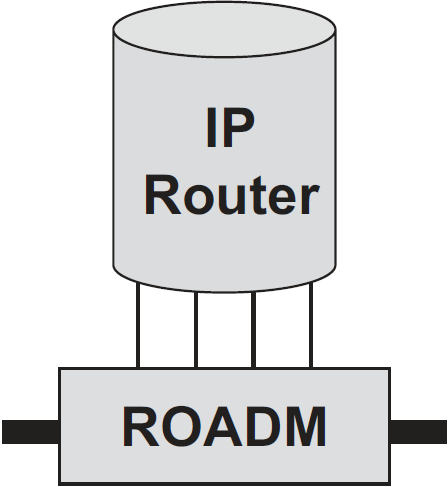
\includegraphics[width=30mm]{IP_router}
\end{subfigure}
\begin{subfigure}{0.49\textwidth}
\centering
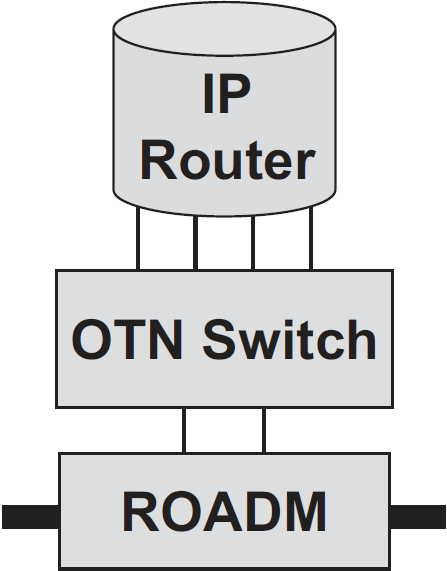
\includegraphics[width=30mm]{IP_OTN}
\end{subfigure}
\end{figure}

\Q

Assume that 135 (identical and independent) services are multiplexed onto a 50GHz wavelength. Each service can be represented by an ON/OFF model, where a service is ON with probability 0.6. When the service is ON, the requested bit rate is 125 Mb/s, deploying PM-QPSK (i.e. four bits per symbol is sent) and sinc pulse shaping.

\begin{enumerate}[label=\alph*-]
\item
What is the probability that the intended offered load exceeds the wavelength capacity? Let $P$ equal this probability.
\item
On average, how full is the 50GHz wavelength?
\item
Next, consider the scenario where these same services are multiplexed onto 10GHz wavelengths. How many services can be multiplexed onto one 10GHz wavelength such that the probability that the intended offered load exceeds the wavelength bit rate is no higher than $P$?
\item
With this number of services on a 10GHz wavelength, on average, how full is the wavelength?
%\item
%What is the statistical multiplexing gain in the 100 Gb/s scenario versus the 10 Gb/s scenario (for the level of P calculated above)?
\end{enumerate}

%\end{enumerate}
\end{document}


